
\chapter{Sprint 1\&2 : Authentification , Gestion des comptes \&  Profil , Gestion des utilisateurs }
\minitoc

\DeclareRobustCommand{\greencheck}{%
  \tikz\fill[scale=0.4, color=green]
  (0,.35) -- (.25,0) -- (1,.7) -- (.25,.15) -- cycle;%
}


\section*{Introduction}
\addcontentsline{toc}{section}{Introduction}
Suite à l’analyse des besoins, ce chapitre présente le lancement du projet SafeTrack selon une approche Agile par sprints.
Les deux premiers sprints portent sur les fonctionnalités essentielles, notamment l’authentification, la gestion des comptes, des profils et des utilisateurs.
Ils constituent la base de l’application et introduisent les principaux artefacts de conception et de réalisation.


\section{Sprint 1 : Authentification \& Gestion des comptes}

L’objectif de ce premier sprint est de mettre en place les fonctionnalités fondamentales permettant à l’utilisateur d’accéder à l’application SafeTrack de manière sécurisée. Ce sprint constitue une étape essentielle, car il assure la gestion des accès, l’authentification des utilisateurs ainsi que la protection des données personnelles.

Les fonctionnalités développées incluent la création de compte (inscription), l’authentification via une interface de connexion, la gestion des sessions sécurisées à l’aide de tokens (JWT), ainsi que la possibilité de réinitialiser le mot de passe en cas d’oubli. Une attention particulière est accordée à la validation des formulaires afin de garantir l’intégrité et la fiabilité des données saisies.

À l’issue de ce sprint, les utilisateurs doivent être en mesure de s’inscrire, de se connecter et d’accéder à leur espace personnel de manière sécurisée, constituant ainsi la base nécessaire à l’utilisation des autres fonctionnalités de l’application.

\subsection{Backlog Sprint 1 :}

Le tableau ci-dessous présente les user stories liées à l’authentification et à la gestion des comptes utilisateurs. Ce sprint vise à mettre en place les mécanismes d’accès sécurisé à l’application SafeTrack, aussi bien pour les utilisateurs mobiles que pour les administrateurs via une interface web dédiée.

\begin{table}[H]
    \caption{Tableau des User Stories – Sprint 1}
\centering
\footnotesize
\setlength{\tabcolsep}{2pt}
\renewcommand{\arraystretch}{0.9}
\setlength{\parskip}{0pt}
\begin{tabularx}{\textwidth}{|c|>{\raggedright\arraybackslash}X|>{\raggedright\arraybackslash}X|c|}
\hline
\textbf{ID} & \textbf{User Story} & \textbf{Tâches} & \textbf{Estimation} \\
\hline

US-01 & En tant que visiteur, je peux m'inscrire via un formulaire en choisissant mon rôle (parent/aidant ou organisation) afin de créer un compte adapté à mon profil.
& \begin{minipage}[t]{\linewidth}\setlength{\itemsep}{-3pt}
{\small
\begin{itemize}[leftmargin=*]
\item Concevoir l'interface d'inscription (mobile et web)
\item Permettre le choix du rôle lors de l'inscription
\item Gérer l'inscription des organisations
\item Implémenter l'API d'inscription (signup)
\item Validation des champs (frontend/backend)
\item Hashage sécurisé du mot de passe (bcrypt)
\item Stockage des données utilisateur
\end{itemize}
}
\end{minipage}
& 3 jours \\
\hline

US-02 & En tant qu'utilisateur, je peux me connecter de manière sécurisée à l’application mobile.
& \begin{minipage}[t]{\linewidth}\setlength{\itemsep}{-3pt}
{\small
\begin{itemize}[leftmargin=*]
\item Concevoir l'interface de connexion (mobile)
\item Implémenter l'API de connexion (login)
\item Génération et gestion des tokens JWT
\item Gestion des erreurs d'authentification
\end{itemize}
}
\end{minipage}
& 3 jours \\
\hline

US-03 & En tant qu'administrateur, je peux me connecter via l’interface web afin d’accéder au tableau de bord d’administration.
& \begin{minipage}[t]{\linewidth}\setlength{\itemsep}{-3pt}
{\small
\begin{itemize}[leftmargin=*]
\item Implémenter l'API de connexion admin
\item Vérification du rôle (admin)
\item Sécurisation de l'accès au dashboard web
\item Interface de connexion web (admin)
\end{itemize}
}
\end{minipage}
& 2 jours \\
\hline

US-04 & En tant qu'utilisateur, je peux me déconnecter.
& \begin{minipage}[t]{\linewidth}\setlength{\itemsep}{-3pt}
{\small
\begin{itemize}[leftmargin=*]
\item Implémenter la fonctionnalité logout
\item Suppression du token côté client
\item Redirection vers l'écran de connexion
\end{itemize}
}
\end{minipage}
& 1 jour \\
\hline

US-05 & En tant qu'utilisateur, je peux réinitialiser mon mot de passe en cas d’oubli.
& \begin{minipage}[t]{\linewidth}\setlength{\itemsep}{-3pt}
{\small
\begin{itemize}[leftmargin=*]
\item Interface "mot de passe oublié"
\item Génération d'un token de réinitialisation sécurisé
\item Envoi d'email de récupération
\item Mise à jour du mot de passe
\end{itemize}
}
\end{minipage}
& 2 jours \\
\hline

US-06 & En tant qu'utilisateur, je peux rester connecté afin de faciliter l’accès à l’application.
& \begin{minipage}[t]{\linewidth}\setlength{\itemsep}{-3pt}
{\small
\begin{itemize}[leftmargin=*]
\item Implémentation des tokens JWT (access/refresh)
\item Stockage sécurisé des tokens (secure storage)
\item Gestion de l'expiration et du renouvellement de session
\end{itemize}
}
\end{minipage}
& 2 jours \\
\hline

US-07 & En tant que système, je dois sécuriser les accès et les données utilisateurs afin de garantir la confidentialité et l’intégrité des informations.
& \begin{minipage}[t]{\linewidth}\setlength{\itemsep}{-3pt}
{\small
\begin{itemize}[leftmargin=*]
\item Sécurisation des routes (Auth Guards)
\item Validation des requêtes
\item Protection contre les attaques (XSS, injection)
\item Tests de sécurité de base
\end{itemize}
}
\end{minipage}
& 2 jours \\
\hline

\end{tabularx}
\end{table}


\subsection{Diagrammes du Sprint 1}
\subsubsection{Diagramme de cas d’utilisation }
La figure \ref{fig:cas_image} présente le diagramme des cas d’utilisation du Sprint 1. 
Ce diagramme illustre les principales interactions entre l’utilisateur et les fonctionnalités liées à l’authentification et à la gestion des comptes.
\begin{figure}[H]
    \centering
    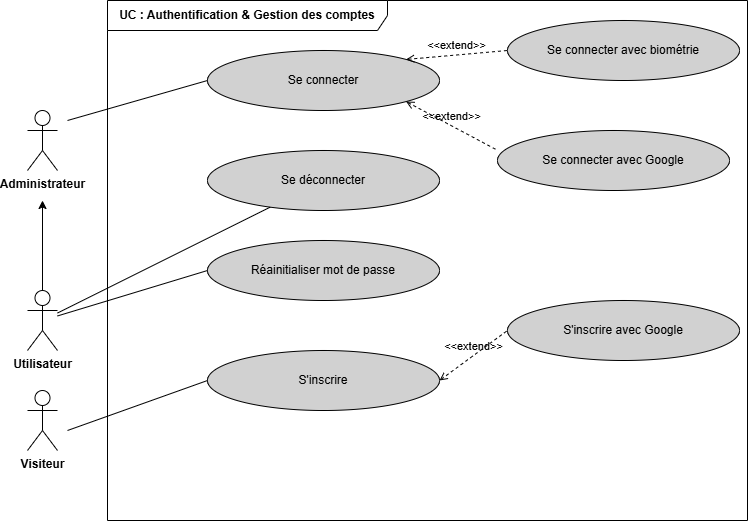
\includegraphics[width=0.9\textwidth]{images/authentification User case.png}
    \caption{Diagramme de cas d'utilisation de sprint 1}
    \label{fig:cas_image}
\end{figure}

\subsubsection{Cas d'utilisation : S'inscrire}

Le cas d'utilisation \og S'inscrire \fg{} est décrit ci‑dessous. Il présente les étapes par lesquelles un visiteur crée un compte SafeTrack, les contrôles effectués (validation des champs, vérification d'unicité) et les conditions d'acceptation.

\small
\renewcommand{\arraystretch}{1.1}
\setlength{\parskip}{0pt}
\begin{longtable}{|p{0.25\textwidth}|>{\raggedright\arraybackslash}p{0.70\textwidth}|}
\caption{Description textuelle du cas d'utilisation S'inscrire} \\
\hline
\textbf{Élément} & \textbf{Description} \\ \hline
\endfirsthead

\hline
\textbf{Élément} & \textbf{Description} \\ \hline
\endhead

\hline
\endlastfoot

Cas d'utilisation & S'inscrire \\ \hline

Acteurs & Visiteur \\ \hline

Précondition & Le visiteur ne possède pas encore de compte sur l'application. \\ \hline

Postcondition & Un compte est créé selon le rôle choisi et les informations sont enregistrées de manière sécurisée. \\ \hline

Scénario nominal &
\begin{itemize}
\item Le visiteur accède au formulaire d'inscription.
\item Le système demande au visiteur de choisir un rôle (Parent/Aidant ou Organisation).
\item Le système affiche les champs requis selon le rôle sélectionné.
\item Le visiteur saisit les informations demandées.
\item Le système valide les données (format de l’email, mot de passe, etc.).
\item Le système vérifie l’unicité de l’adresse email.
\item Si les informations sont valides, le système crée le compte correspondant au rôle choisi.
\item Le visiteur reçoit une confirmation d’inscription.
\end{itemize}
\\ \hline

Scénario alternatif &
\begin{itemize}
\item \textbf{Email déjà utilisé :}
\begin{itemize}
\item Le système détecte l'existence d’un compte associé à l’adresse email.
\item Un message d’erreur est affiché.
\end{itemize}

\item \textbf{Mot de passe non conforme :}
\begin{itemize}
\item Le mot de passe ne respecte pas les règles de sécurité.
\item Le système demande une correction.
\end{itemize}

\item \textbf{Données incomplètes :}
\begin{itemize}
\item Certains champs obligatoires sont manquants.
\item Le système empêche la création du compte et signale les erreurs.
\end{itemize}
\end{itemize}
\\ \hline

\end{longtable}
\subsubsection{Diagramme de séquence de \og S'inscrire \fg}

La figure~\ref{fig:chap3_signup_sequence} illustre le diagramme de séquence du cas d'utilisation \og S'inscrire \fg{} pour le scénario nominal. Les interactions couvrent la saisie des données, leur validation et la création du compte utilisateur.

\begin{figure}[H]
    \centering
    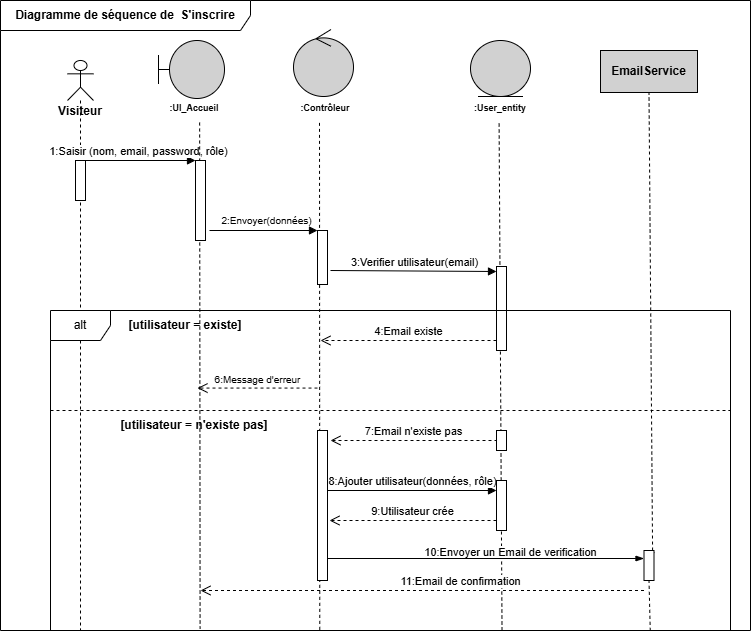
\includegraphics[width=\textwidth, height=1\textheight, keepaspectratio]{images/DS s'inscrire.png}
    \caption{Diagramme de séquence de S'inscrire}
    \label{fig:chap3_signup_sequence}
\end{figure}

\subsubsection{Cas d'utilisation : S'authentifier}

Le cas d'utilisation \og S'authentifier \fg{} est présenté ci‑dessous. Cette description couvre l'ensemble des méthodes d'accès au système SafeTrack : 
authentification classique par email et mot de passe, authentification biométrique, 
et authentification via Google OAuth.

\small
\renewcommand{\arraystretch}{1.1}
\setlength{\parskip}{0pt}
\begin{longtable}{|p{0.25\textwidth}|>{\raggedright\arraybackslash}p{0.70\textwidth}|}
\caption{Description textuelle du cas d'utilisation S'authentifier} \\
\hline
\textbf{Élément} & \textbf{Description} \\ \hline
\endfirsthead

\hline
\textbf{Élément} & \textbf{Description} \\ \hline
\endhead

\hline
\endlastfoot

Cas d'utilisation & S'authentifier \\ \hline

Acteurs & Utilisateur (Parent / Enfant), Administrateur \\ \hline

Précondition & L'acteur possède un compte valide et peut s'authentifier via mot de passe, biométrie ou Google OAuth. \\ \hline

Postcondition & L'acteur est authentifié et accède à son espace sécurisé selon son rôle. \\ \hline

Scénario nominal &
\begin{itemize}
\item L'acteur accède à l'interface de connexion.
\item Le système propose : e-mail/mot de passe, biométrie ou Google.
\item L'acteur choisit une méthode :
\begin{itemize}
\item Authentification classique : saisie et vérification.
\item Biométrie : validation de l'empreinte.
\item Google OAuth : authentification via Google.
\end{itemize}
\item Le système génère les tokens d'accès.
\item L'acteur accède à son tableau de bord.
\end{itemize}
\\ \hline

Scénario alternatif &
\begin{itemize}
\item \textbf{Mot de passe oublié :}
\begin{itemize}
\item Saisie de l’e-mail.
\item Réception d’un lien de réinitialisation.
\item Définition d’un nouveau mot de passe.
\end{itemize}

\item \textbf{Renouvellement de session :}
\begin{itemize}
\item Expiration du token.
\item Utilisation du refresh token.
\item Génération d’un nouveau token.
\end{itemize}

\item \textbf{Erreurs d’authentification :}
\begin{itemize}
\item Identifiants incorrects.
\item Échec biométrique.
\item Compte non lié ou non vérifié.
\item Erreur système.
\end{itemize}
\end{itemize}
\\ \hline

\end{longtable}
\subsubsection{Diagramme de séquence de \og S'authentifier \fg}

La figure~\ref{fig:chap3_auth_sequence} illustre le diagramme de séquence du cas d'utilisation \og S'authentifier \fg{} pour le scénario nominal A (authentification classique). Les scénarios B (biométrique) et C (Google) suivent des flux similaires avec des étapes de validation spécifiques.

\begin{figure}[H]
    \centering
    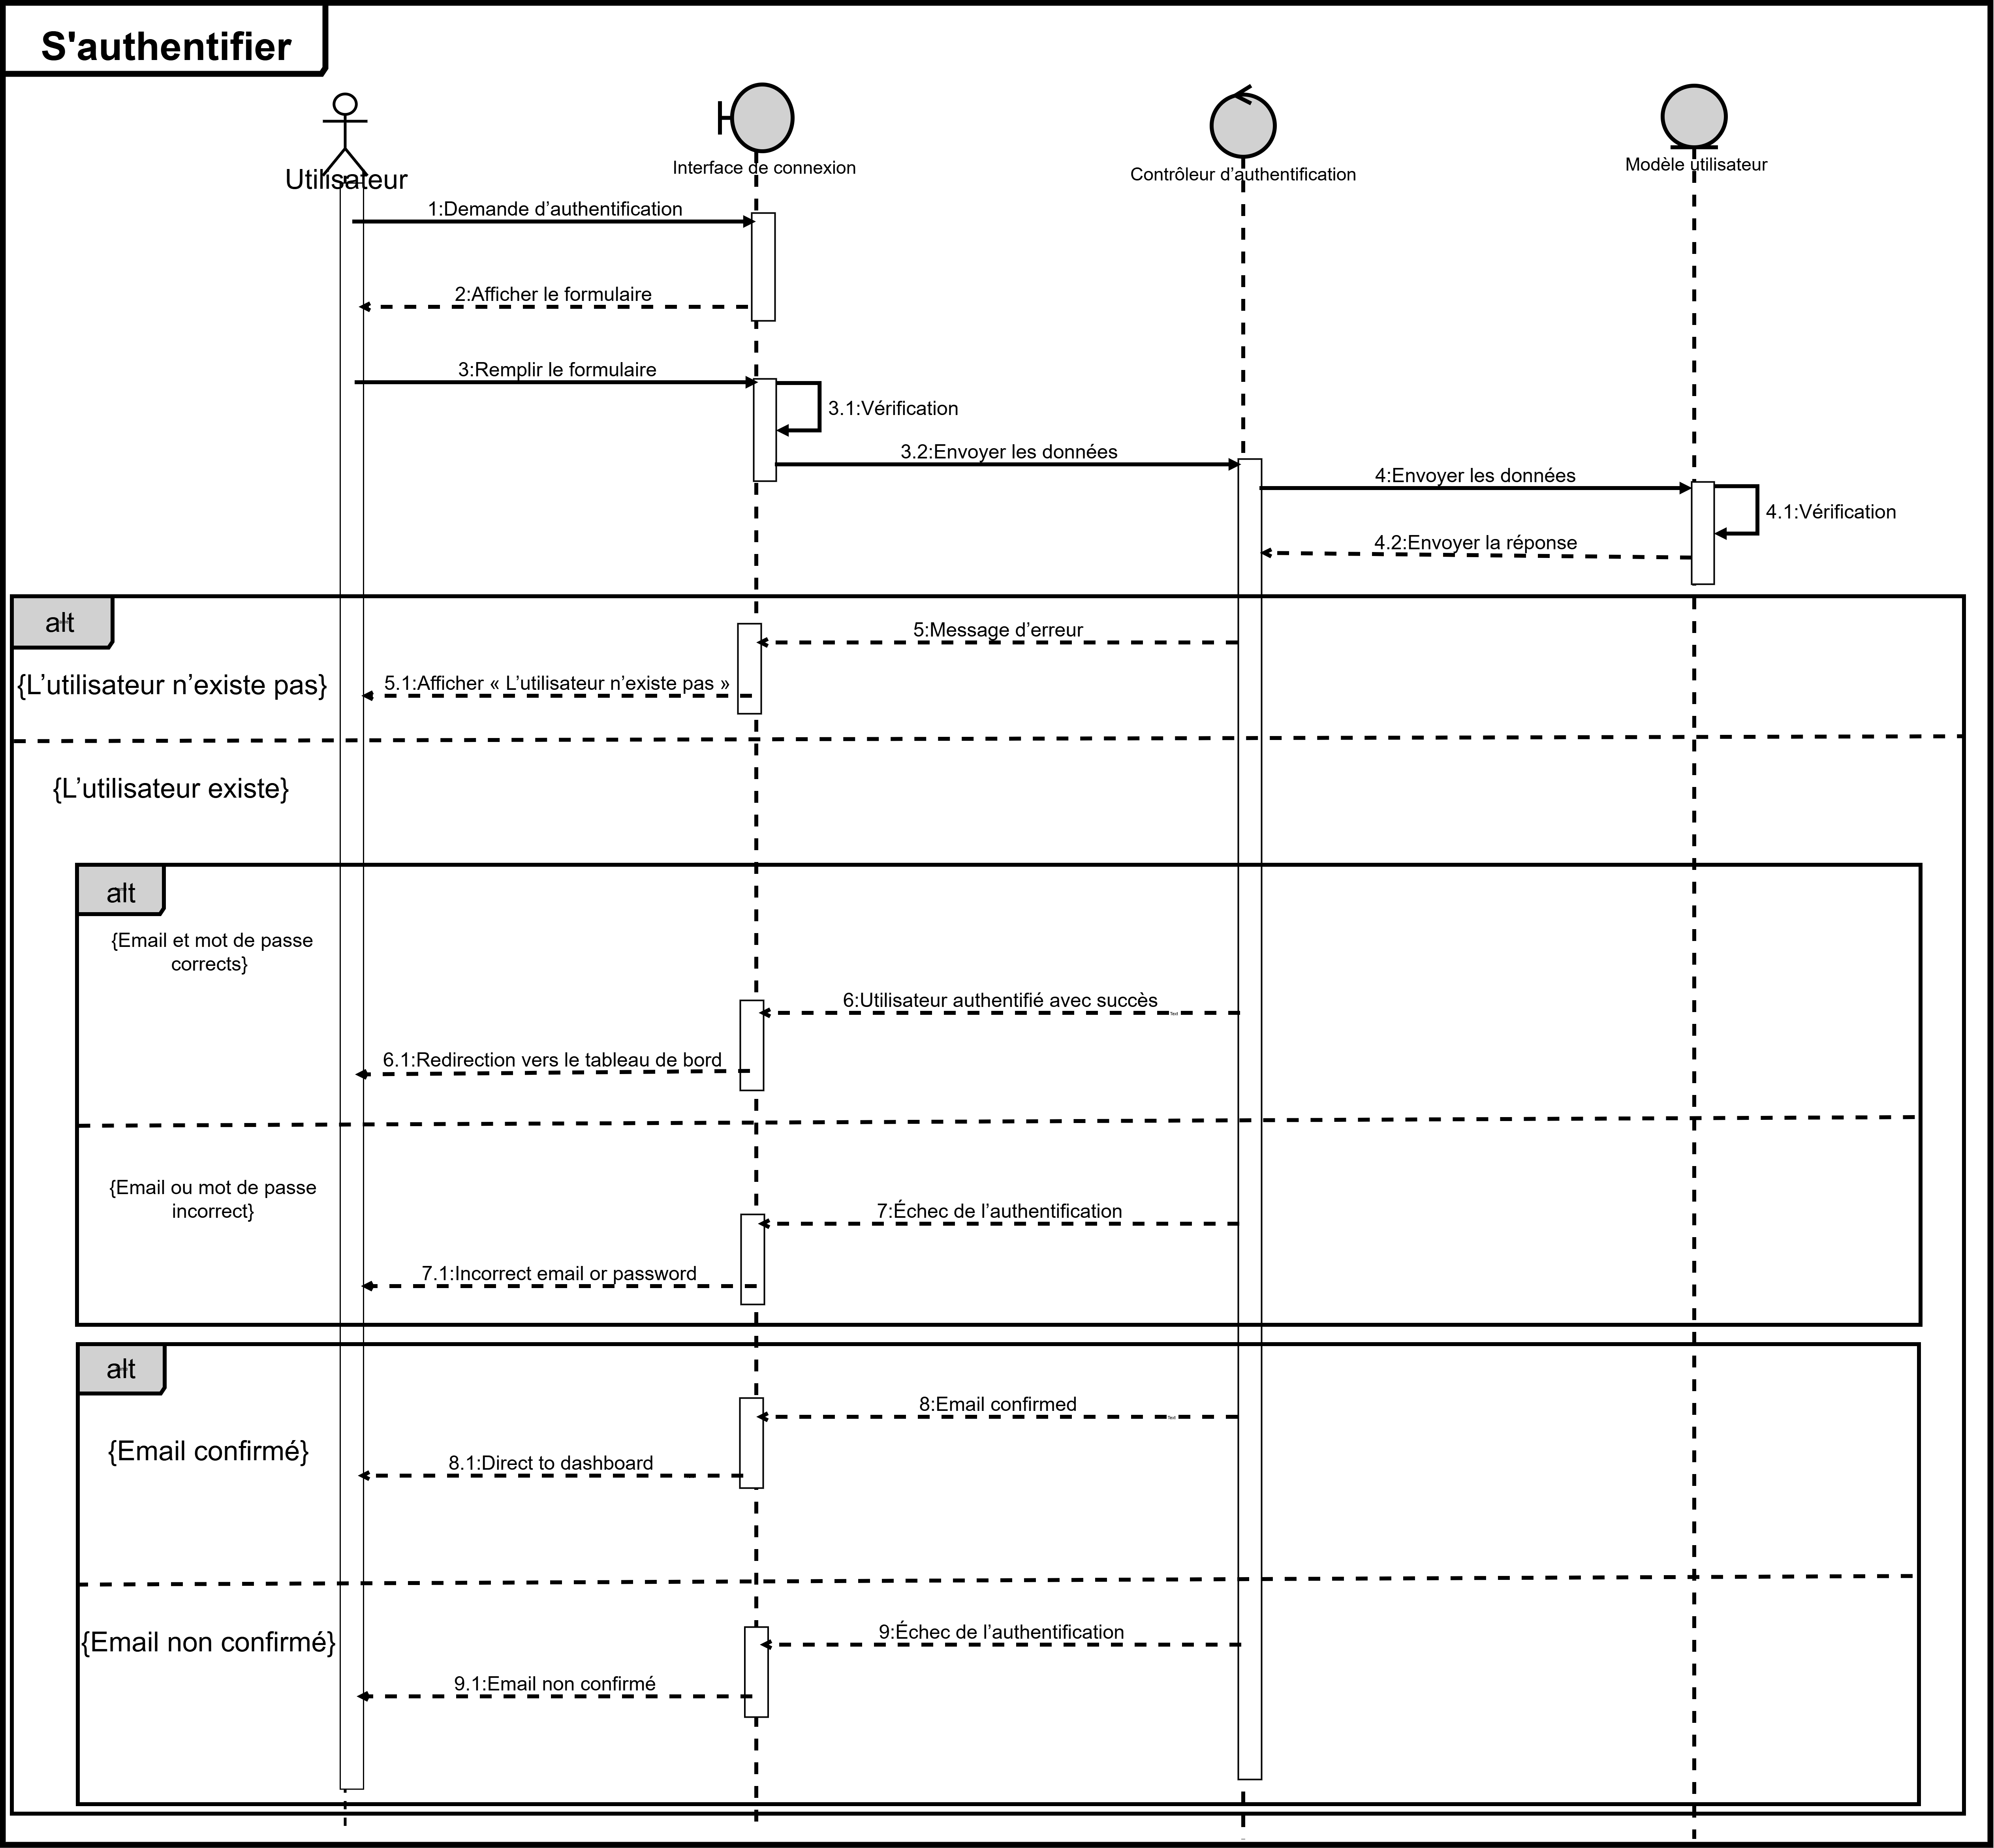
\includegraphics[width=\textwidth, height=1\textheight, keepaspectratio]{images/Sq_auth.drawio.png
    }
    \caption{Diagramme de séquence de S'authentifier (scénario classique)}
    \label{fig:chap3_auth_sequence}
\end{figure}
\subsection{Réalisation du Sprint 1:}

\subsubsection{Réalisation du cas d’utilisation : S’inscrire}

Pour s’inscrire dans l’application \textit{SafeTrack}, l’utilisateur commence par remplir le formulaire d’inscription (nom, email, mot de passe, etc.) depuis l’interface mobile ou web.

Les données saisies sont envoyées au backend via l’API d’inscription. Le système procède ensuite à plusieurs vérifications :

\begin{itemize}
    \item validation du format de l’email,
    \item contrôle de la conformité du mot de passe (longueur minimale et règles de sécurité),
    \item vérification de l’unicité de l’email dans la base de données.
\end{itemize}

Si toutes les vérifications sont réussies, le système crée un nouveau compte utilisateur et enregistre les informations de manière sécurisée dans la base de données.

\subsubsection{Réalisation du cas d’utilisation : S’authentifier}

Pour se connecter, l’utilisateur saisit son email et son mot de passe dans l’interface de connexion.

Les informations sont envoyées au backend, où le système :

\begin{itemize}
    \item vérifie l’existence de l’utilisateur,
    \item compare le mot de passe fourni avec celui stocké (haché),
    \item génère un token d’authentification (JWT) en cas de succès.
\end{itemize}

Ce token permet à l’utilisateur d’accéder aux fonctionnalités protégées de l’application de manière sécurisée, sans avoir à se reconnecter à chaque requête.


\section{Sprint 2 : Profil \& Gestion des utilisateurs}

Ce deuxième sprint vise à améliorer l’expérience utilisateur en introduisant les fonctionnalités liées à la gestion du profil et des contacts. Il permet principalement aux acteurs responsables (parents, aidants ou organisations) de personnaliser leurs informations et de gérer les relations avec les personnes suivies dans l’application SafeTrack.

Les fonctionnalités développées incluent la consultation et la modification des informations du profil (nom, prénom, coordonnées, etc.), ainsi que la gestion des contacts (ajout, suppression et consultation). Ces actions sont réservées aux utilisateurs disposant des droits appropriés, notamment les parents, les aidants ou les organisations. 

En revanche, les personnes vulnérables disposent uniquement d’un accès limité en consultation, sans possibilité de modifier leur profil ou de gérer des contacts.

À la fin de ce sprint, l’application offre un espace utilisateur personnalisable et permet d’établir un réseau de confiance entre les différents acteurs, ce qui constitue une base essentielle pour les fonctionnalités de suivi, de localisation et d’alertes développées dans les sprints suivants.



\subsection{Backlog Sprint 2 :}

La gestion et la personnalisation du profil utilisateur représentent un aspect essentiel d’une application orientée sécurité. Les user stories suivantes décrivent les fonctionnalités permettant aux acteurs autorisés (parents, aidants ou organisations) de gérer les profils et les contacts.

\begin{table}[H]
    \caption{Backlog Sprint 2 – Gestion des profils et contacts}
\centering
\small
\setlength{\tabcolsep}{3pt}
\renewcommand{\arraystretch}{1.0}
\setlength{\parskip}{0pt}
\begin{tabularx}{\textwidth}{|c|>{\raggedright\arraybackslash}X|>{\raggedright\arraybackslash}X|c|}
\hline
\textbf{ID} & \textbf{User Story} & \textbf{Tâches} & \textbf{Estimation} \\
\hline

US-010 & En tant qu'utilisateur, je peux consulter mon profil afin de visualiser mes informations personnelles.
& \begin{minipage}[t]{\linewidth}\setlength{\itemsep}{-2pt}
\begin{itemize}[leftmargin=*]
\item Interface profil
\item API récupération données
\item Affichage infos utilisateur
\end{itemize}
\end{minipage}
& 2 jours \\
\hline

US-011 & En tant que parent/aidant/organisation, je peux modifier mon profil afin de mettre à jour mes informations personnelles.
& \begin{minipage}[t]{\linewidth}\setlength{\itemsep}{-2pt}
\begin{itemize}[leftmargin=*]
\item Formulaire modification
\item Upload photo
\item API mise à jour profil
\end{itemize}
\end{minipage}
& 3 jours \\
\hline

US-012 & En tant que parent/aidant, je peux ajouter un contact afin d’étendre mon réseau de confiance.
& \begin{minipage}[t]{\linewidth}\setlength{\itemsep}{-2pt}
\begin{itemize}[leftmargin=*]
\item Formulaire ajout contact
\item API ajout
\item Validation des données
\end{itemize}
\end{minipage}
& 2 jours \\
\hline

US-013 & En tant que parent/aidant, je peux supprimer un contact afin de gérer mon réseau.
& \begin{minipage}[t]{\linewidth}\setlength{\itemsep}{-2pt}
\begin{itemize}[leftmargin=*]
\item Bouton suppression
\item Confirmation action
\item API suppression
\end{itemize}
\end{minipage}
& 1 jour \\
\hline

US-014 & En tant que parent/aidant, je peux consulter la liste des contacts associés.
& \begin{minipage}[t]{\linewidth}\setlength{\itemsep}{-2pt}
\begin{itemize}[leftmargin=*]
\item Interface liste contacts
\item API récupération
\item Affichage liste
\end{itemize}
\end{minipage}
& 2 jours \\
\hline

US-015 & En tant que parent/aidant, je peux consulter les détails d’un contact.
& \begin{minipage}[t]{\linewidth}\setlength{\itemsep}{-2pt}
\begin{itemize}[leftmargin=*]
\item Page détail contact
\item Affichage informations
\item Navigation
\end{itemize}
\end{minipage}
& 1 jour \\
\hline

US-016 & En tant qu’utilisateur, je peux recevoir un retour visuel lors d’une action afin d’améliorer l’expérience utilisateur.
& \begin{minipage}[t]{\linewidth}\setlength{\itemsep}{-2pt}
\begin{itemize}[leftmargin=*]
\item Messages de confirmation
\item Notifications UI
\item Gestion du feedback utilisateur
\end{itemize}
\end{minipage}
& 1 jour \\
\hline

US-017 & En tant que parent/aidant, je peux rechercher un contact afin de le retrouver rapidement.
& \begin{minipage}[t]{\linewidth}\setlength{\itemsep}{-2pt}
\begin{itemize}[leftmargin=*]
\item Barre de recherche
\item Filtrage de la liste
\item Optimisation de la recherche
\end{itemize}
\end{minipage}
& 2 jours \\

\hline
\end{tabularx}
\end{table}


\subsection{Diagrammes du Sprint 2}
\subsubsection{Diagramme de cas d’utilisation }
La figure \ref{fig:chap3_sprint2} présente le diagramme des cas d’utilisation du Sprint 2. 
Ce diagramme illustre les principales interactions entre l’utilisateur et les fonctionnalités liées à la gestion du profil et des contacts dans l’application SafeTrack.
\begin{figure}[H]
    \centering
    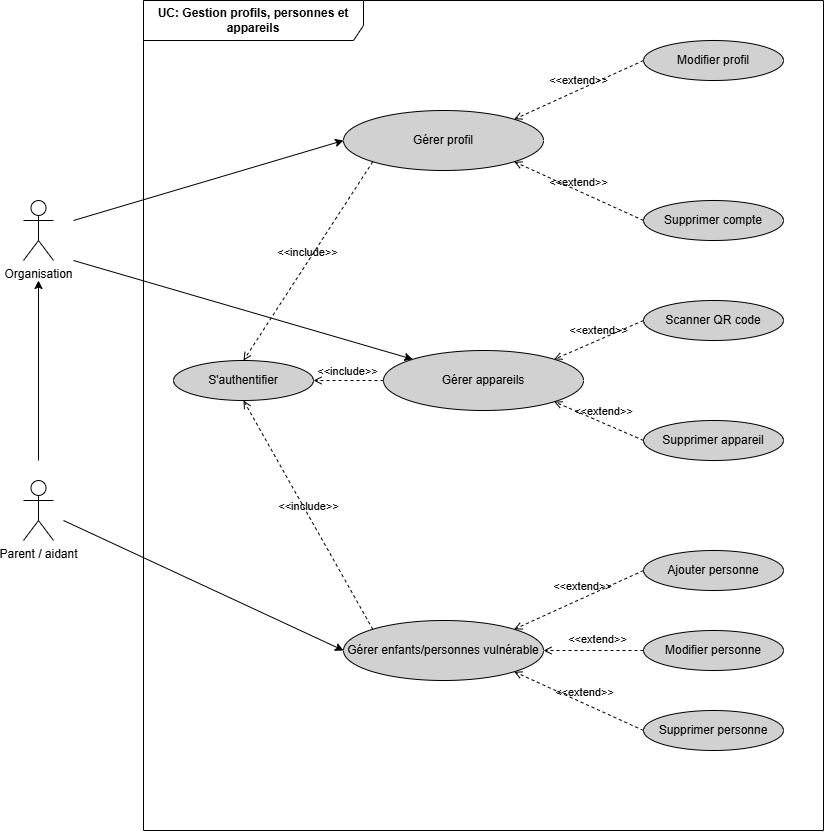
\includegraphics[width=0.9\textwidth]{images/UC_sprint2.png}
    \caption{Diagramme de cas d'utilisation de sprint2}
    \label{fig:chap3_sprint2}
\end{figure}


\subsubsection{Cas d'utilisation : Modifier profil}

Le cas d'utilisation \og Modifier profil \fg{} est présenté ci‑dessous. Cette description couvre l'ensemble des opérations permettant à l'utilisateur de mettre à jour ses informations personnelles.

\small
\renewcommand{\arraystretch}{1.1}
\setlength{\parskip}{0pt}
\begin{longtable}{|p{0.25\textwidth}|>{\raggedright\arraybackslash}p{0.70\textwidth}|}
\caption{Description textuelle du cas d'utilisation Modifier profil} \\
\hline
\textbf{Élément} & \textbf{Description} \\ \hline
\endfirsthead

\hline
\textbf{Élément} & \textbf{Description} \\ \hline
\endhead

\hline
\endlastfoot

Cas d'utilisation & Modifier profil \\ \hline

Acteurs & Parent, Aidant, Organisation, Enfant/Personne vulnérable \\ \hline

Précondition & L'utilisateur est authentifié, possède un compte actif et dispose des permissions de modification de profil (son propre profil ou celui de ses enfants/personnes vulnérables associées). \\ \hline

Postcondition & Les modifications du profil sont enregistrées dans la base de données et l'utilisateur en reçoit une confirmation. \\ \hline

Scénario nominal &
\begin{itemize}
\item L'utilisateur accède à son espace profil ou sélectionne un enfant/personne vulnérable.
\item Le système affiche le formulaire de modification avec les données actuelles.
\item L'utilisateur édite les champs souhaités (nom, email, téléphone, permissions, etc.).
\item L'utilisateur peut importer une photo de profil.
\item Le système valide les données saisies.
\item L'utilisateur confirme les modifications.
\item Les nouvelles données sont enregistrées en base de données.
\item L'utilisateur reçoit un message de confirmation.
\end{itemize}
\\ \hline

Scénario alternatif &
\begin{itemize}
\item \textbf{Modification du profil d'un enfant/personne vulnérable :}
\begin{itemize}
\item Parent sélectionne un enfant dans la liste des personnes associées.
\item Modification des informations de l'enfant (restrictions appliquées selon les droits).
\item Modification des permissions et autorisations de l'enfant.
\item Validation et enregistrement des modifications.
\end{itemize}

\item \textbf{Modification de photo :}
\begin{itemize}
\item Upload d'une nouvelle photo de profil.
\item Validation du format (JPEG, PNG) et de la taille (max 5MB).
\item Remplacement de l'ancienne photo ou première importation.
\end{itemize}

\item \textbf{Restrictions d'accès :}
\begin{itemize}
\item Enfant/personne vulnérable avec accès lecture seule sur son propre profil.
\item Modification possible uniquement par le parent/aidant responsable.
\item Certains champs non modifiables par l'enfant (permissions, alertes, etc.).
\end{itemize}

\item \textbf{Erreurs de validation :}
\begin{itemize}
\item Format email invalide.
\item Numéro de téléphone non valide.
\item Champs obligatoires manquants.
\item Message d'erreur spécifique avec suggestion de correction.
\end{itemize}
\end{itemize}
\\ \hline

\end{longtable}

\subsubsection{Diagramme de séquence de \og Modifier profil \fg}

La figure~\ref{fig:chap3_profile_modify_sequence} illustre le diagramme de séquence du cas d'utilisation \og Modifier profil \fg{} pour le scénario nominal. Les interactions couvrent la récupération des données actuelles, la validation des modifications et l'enregistrement en base de données.

\begin{figure}[H]
    \centering
    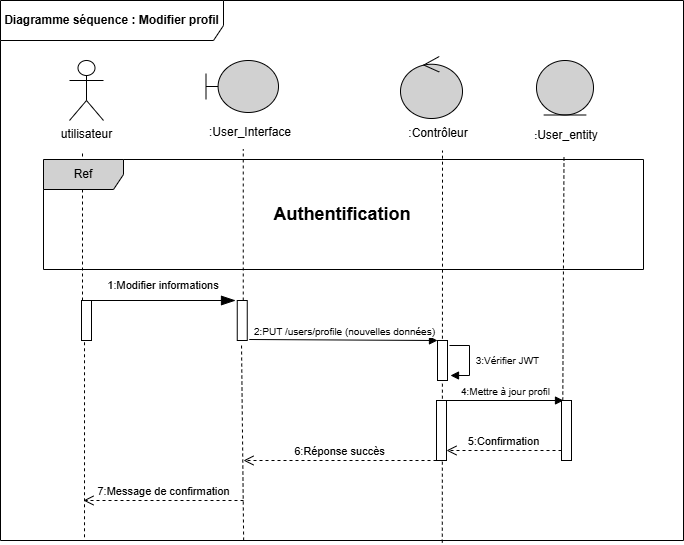
\includegraphics[width=\textwidth, height=1\textheight, keepaspectratio]{images/modifierProfil_S2.drawio.png}
    \caption{Diagramme de séquence de Modifier profil}
    \label{fig:chap3_profile_modify_sequence}
\end{figure}

\subsubsection{Cas d'utilisation : Ajouter un enfant/personne vulnérable}

Le cas d'utilisation \og Ajouter un enfant/personne vulnérable \fg{} est présenté ci‑dessous. Cette description couvre l'ensemble des opérations permettant aux parents/aidants de créer un profil pour un enfant ou une personne vulnérable et de générer automatiquement ses identifiants d'accès.

\small
\renewcommand{\arraystretch}{1.1}
\setlength{\parskip}{0pt}
\begin{longtable}{|p{0.25\textwidth}|>{\raggedright\arraybackslash}p{0.70\textwidth}|}
\caption{Description textuelle du cas d'utilisation Ajouter un enfant/personne vulnérable} \\
\hline
\textbf{Élément} & \textbf{Description} \\ \hline
\endfirsthead

\hline
\textbf{Élément} & \textbf{Description} \\ \hline
\endhead

\hline
\endlastfoot

Cas d'utilisation & Ajouter un enfant/personne vulnérable \\ \hline

Acteurs & Parent, Aidant \\ \hline

Précondition & L'utilisateur (parent ou aidant) est authentifié, possède un compte actif et dispose des permissions de création d'enfants/personnes vulnérables. \\ \hline

Postcondition & Un nouveau profil enfant/personne vulnérable est créé avec un compte d'accès généré. Les identifiants sont transmis au parent/aidant par email. Le profil est lié au compte du parent et enregistré dans la base de données. \\ \hline

Scénario nominal &
\begin{itemize}
\item L'utilisateur (parent/aidant) accède au module de gestion des enfants.
\item L'utilisateur clique sur le bouton « Ajouter un enfant/personne vulnérable ».
\item Le système affiche un formulaire contenant les champs : nom, email et âge.
\item L'utilisateur remplit les informations requises.
\item Le système valide les données saisies (format email, âge valide, champs obligatoires).
\item Le système génère automatiquement un compte avec un mot de passe sécurisé.
\item Le nouvel enfant/personne vulnérable est enregistré et lié au compte du parent.
\item Le système envoie un email au parent contenant l'adresse email et le mot de passe temporaire du compte de l'enfant.
\item L'utilisateur reçoit une confirmation d'ajout avec les détails du profil créé.
\end{itemize}
\\ \hline

Scénario alternatif &
\begin{itemize}
\item \textbf{Réinitialisation du mot de passe :}
\begin{itemize}
\item Si le parent n'a pas reçu l'email ou souhaite générer un nouveau mot de passe.
\item Sélection de l'enfant dans la liste et option « Réinitialiser le mot de passe ».
\item Génération d'un nouveau mot de passe temporaire.
\item Envoi d'un nouvel email contenant le mot de passe.
\end{itemize}

\item \textbf{Modification du profil enfant :}
\begin{itemize}
\item Après création, le parent peut modifier les informations (nom, âge).
\item Le parent peut configurer les permissions, zones de sécurité et paramètres de suivi.
\item Sauvegarde et confirmation des modifications.
\end{itemize}

\item \textbf{Erreurs ou restrictions :}
\begin{itemize}
\item Email déjà utilisé par un autre profil.
\item Données incomplètes ou invalides (format email, âge invalide).
\item Permissions insuffisantes pour l'ajout.
\item Message d'erreur approprié avec indication de correction.
\end{itemize}
\end{itemize}
\\ \hline

\end{longtable}

\subsubsection{Diagramme de séquence de \og Ajouter un enfant/personne vulnérable \fg}

La figure~\ref{fig:chap3_children_management_sequence} illustre le diagramme de séquence du cas \og Gestion des enfants \fg{} pour le scénario nominal. Les interactions couvrent les opérations d'ajout, consultation, modification et suppression d'enfants/personnes vulnérables.

\begin{figure}[H]
    \centering
    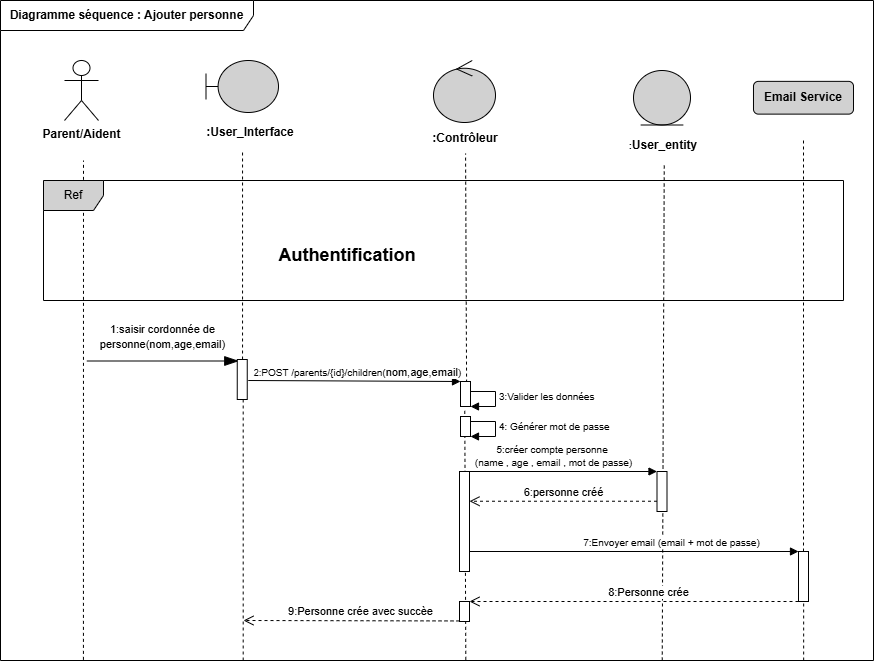
\includegraphics[width=\textwidth, height=1\textheight, keepaspectratio]{images/DS_ Ajouter personne_S2.drawio.png}
    \caption{Diagramme de séquence de Gestion des enfants}
    \label{fig:chap3_children_management_sequence}
\end{figure}



\subsection{Réalisation du Sprint 2 : }

\subsubsection{Réalisation du cas d'utilisation : Modifier profil}

Après authentification, l’utilisateur peut accéder à son espace profil et modifier les informations autorisées.

L’application envoie une requête sécurisée au backend en utilisant le token JWT. Le serveur vérifie l’authenticité du token, récupère les données courantes, valide les modifications soumises puis met à jour la base de données. Les changements sont confimés à l’utilisateur via un message de retour.

Les restrictions d'accès sont respectées : un parent/aidant peut modifier son propre profil et, selon les permissions, les profils des enfants/personnes vulnérables qui lui sont associés.

\subsubsection{Réalisation du cas d'utilisation : Ajouter un enfant/personne vulnérable}

Le module de gestion des enfants permet aux parents/aidants de créer, consulter, modifier et supprimer des profils d'enfants ou de personnes vulnérables.

Fonctionnalités réalisées :

\begin{itemize}
    \item \textbf{Ajout d'un enfant/personne vulnérable :} Le parent/aidant remplit un formulaire simple contenant les champs suivants : nom, email et âge. Le système valide les données saisies (format email valide, âge cohérent, champs obligatoires). Un compte d'accès est créé automatiquement avec un mot de passe sécurisé généré par le système. Le profil de l'enfant est lié au compte du parent et enregistré en base de données. Le parent reçoit un email contenant l'adresse email et le mot de passe temporaire du compte de l'enfant pour son utilisation ultérieure.
    
    \item \textbf{Consultation :} Affichage de la liste complète des enfants/personnes vulnérables associés au parent. Accès à la fiche détaillée de chaque profil incluant les informations personnelles (nom, âge, email), les autorisations, les paramètres de suivi et l'historique des activités.
    
    \item \textbf{Modification :} Le parent/aidant peut modifier les informations de l'enfant (nom, âge) et configurer les permissions, zones de sécurité et paramètres de suivi. Mise à jour des données en base avec validation des changements et confirmation des modifications.
    
    \item \textbf{Réinitialisation du mot de passe :} Si le parent n'a pas reçu l'email initial ou souhaite générer un nouveau mot de passe, il peut accéder à l'option « Réinitialiser le mot de passe » depuis la fiche de l'enfant. Un nouveau mot de passe temporaire est généré et envoyé par email au parent.
    
    \item \textbf{Suppression :} Détachement ou suppression du profil avec confirmation préalable. Un message de confirmation de suppression est affiché en cas de succès, et des messages d'erreur appropriés sont retournés en cas d'échec.
\end{itemize}

Toutes les opérations sont sécurisées et soumises à des contrôles d'autorisation pour prévenir les modifications non autorisées. Seuls les parents/aidants disposant des droits appropriés peuvent accéder à ces fonctionnalités.

\section{Présentation des interface de l'application}
\newpage


\begin{figure}[H]
    \centering

    % First row: Web + Mobile side by side (larger)
    \begin{minipage}[b]{0.6\textwidth}
        \centering
        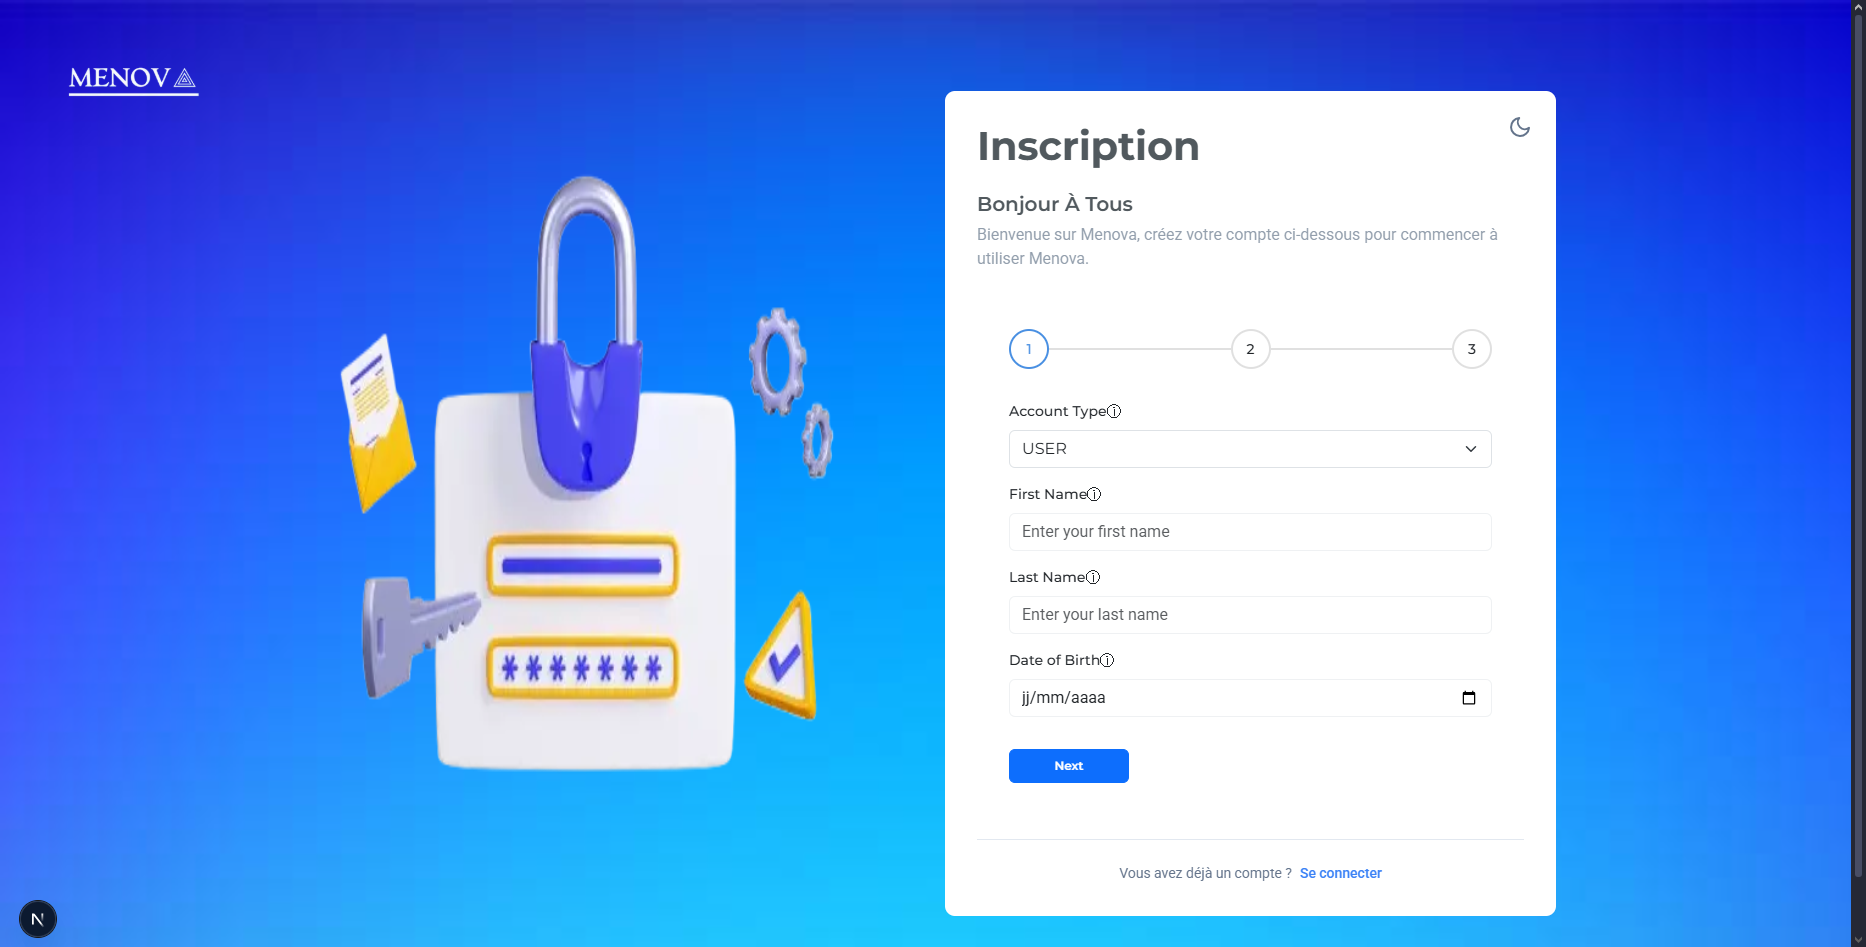
\includegraphics[width=\linewidth, height=0.4\textheight, keepaspectratio]{images/RegisterWeb.png}
        \caption{Interface Web – Inscription Menova – étape 1}
    \end{minipage}
    \hfill
    \begin{minipage}[b]{0.38\textwidth}
        \centering
        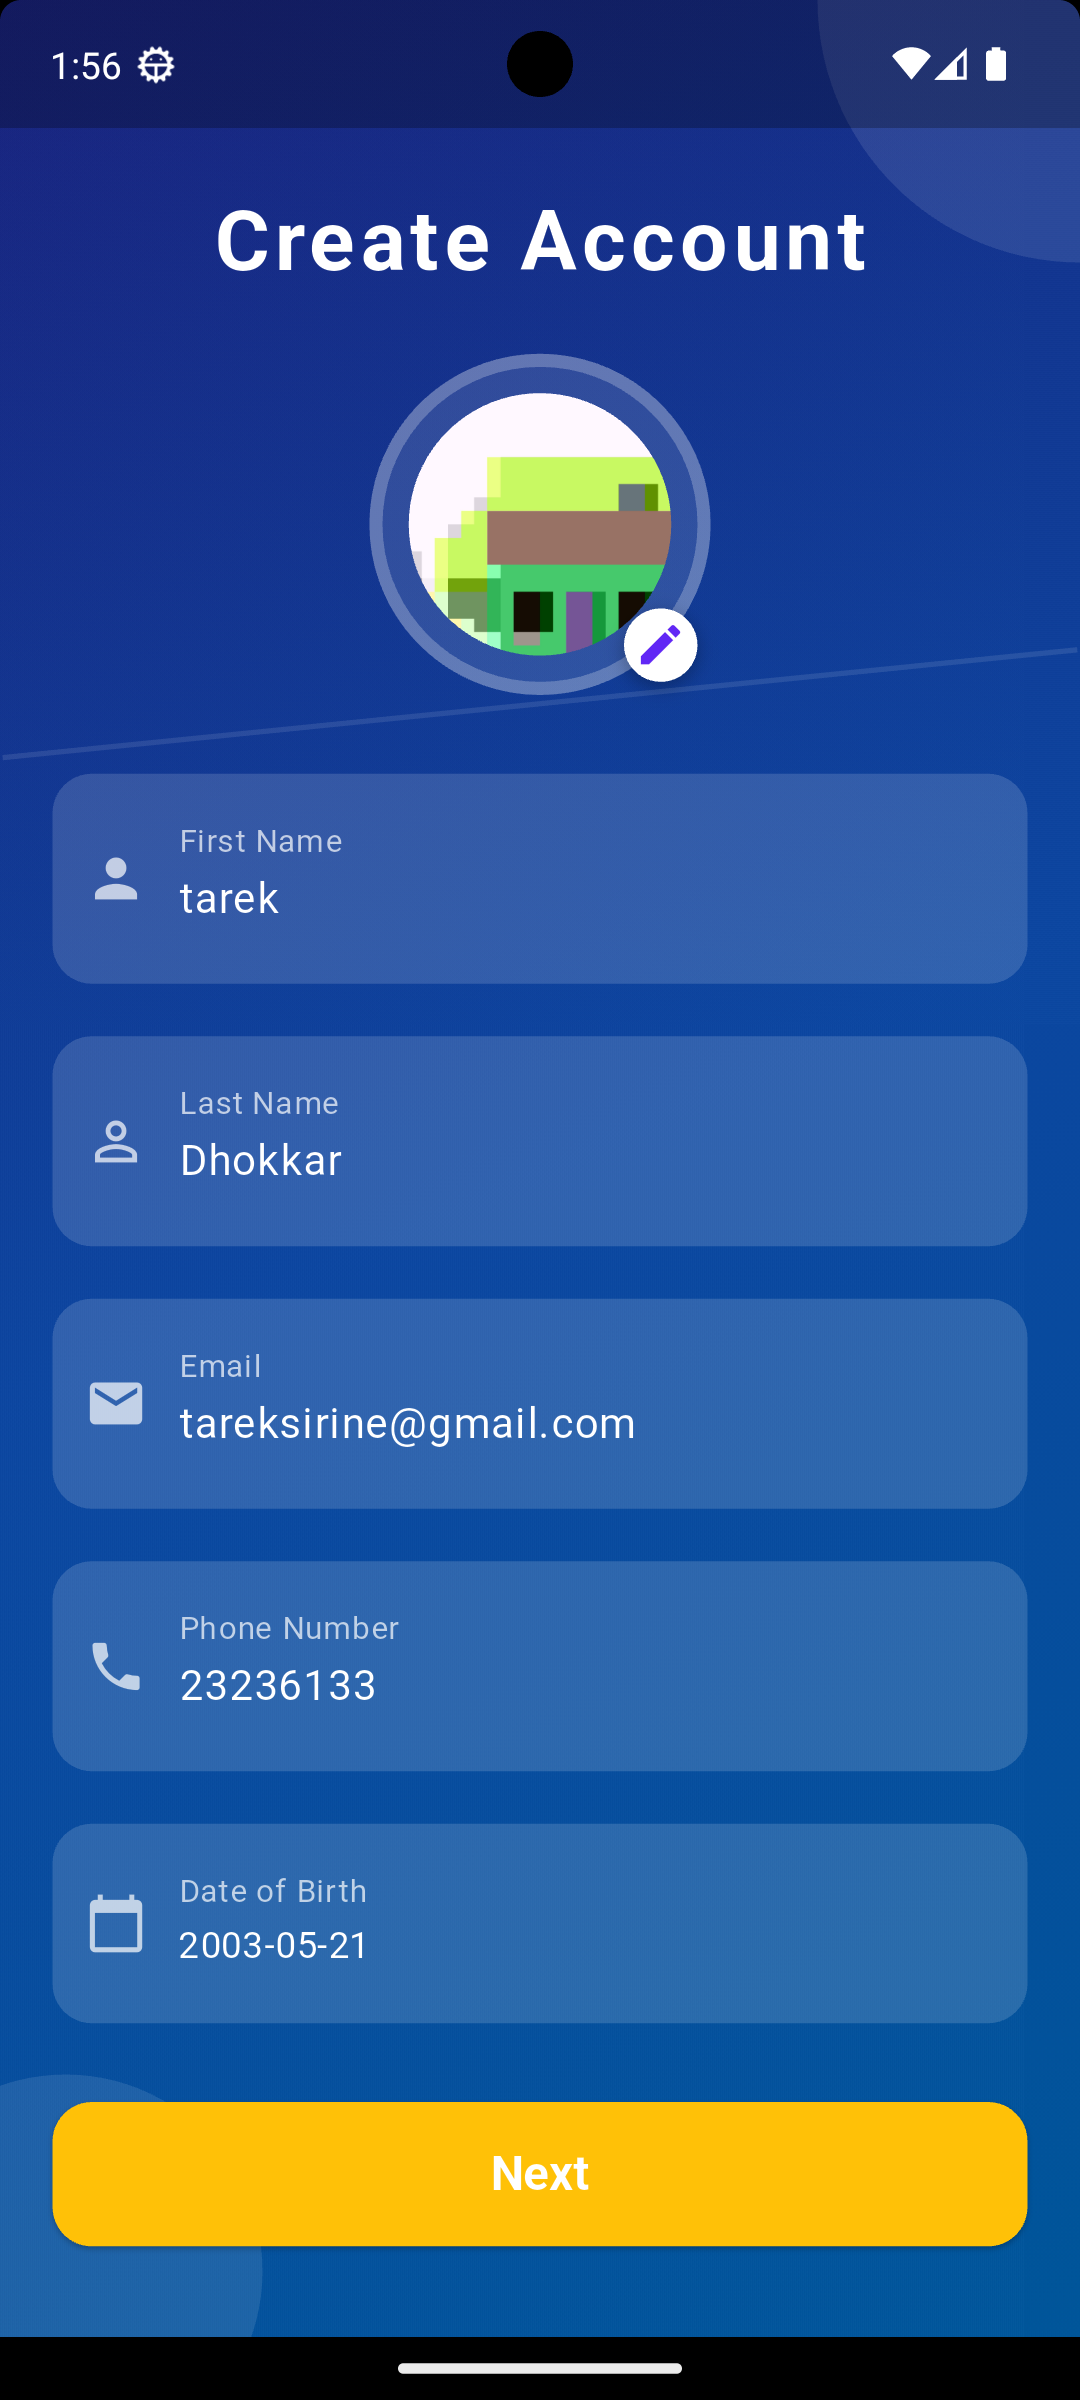
\includegraphics[width=\linewidth, height=0.4\textheight, keepaspectratio]{images/Screenshot_1747835775.png}
        \caption{Interface Mobile – Inscription Menova – étape 1}
    \end{minipage}

    \vspace{1.8em}

    % Second row: Web + Mobile side by side (larger)
    \begin{minipage}[b]{0.6\textwidth}
        \centering
        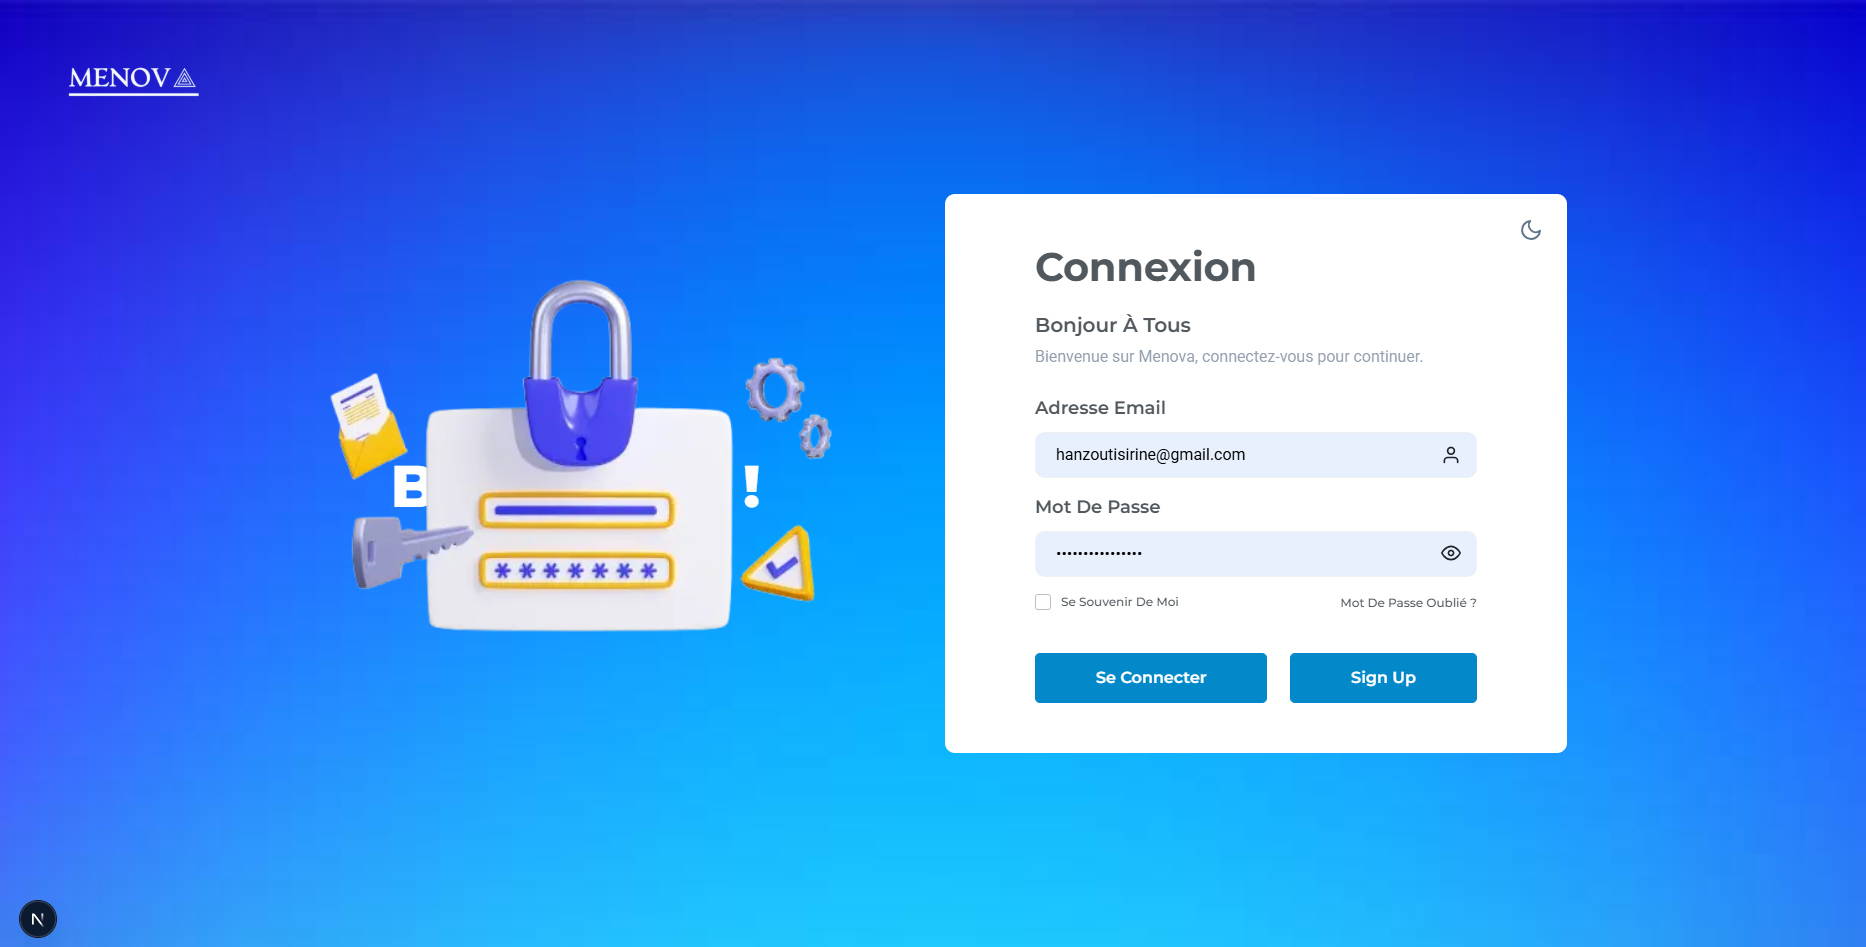
\includegraphics[width=\linewidth, height=0.4\textheight, keepaspectratio]{images/Login.png}
        \caption{Interface Web – Page de connexion Menova – étape 2}
    \end{minipage}
    \hfill
    \begin{minipage}[b]{0.38\textwidth}
        \centering
        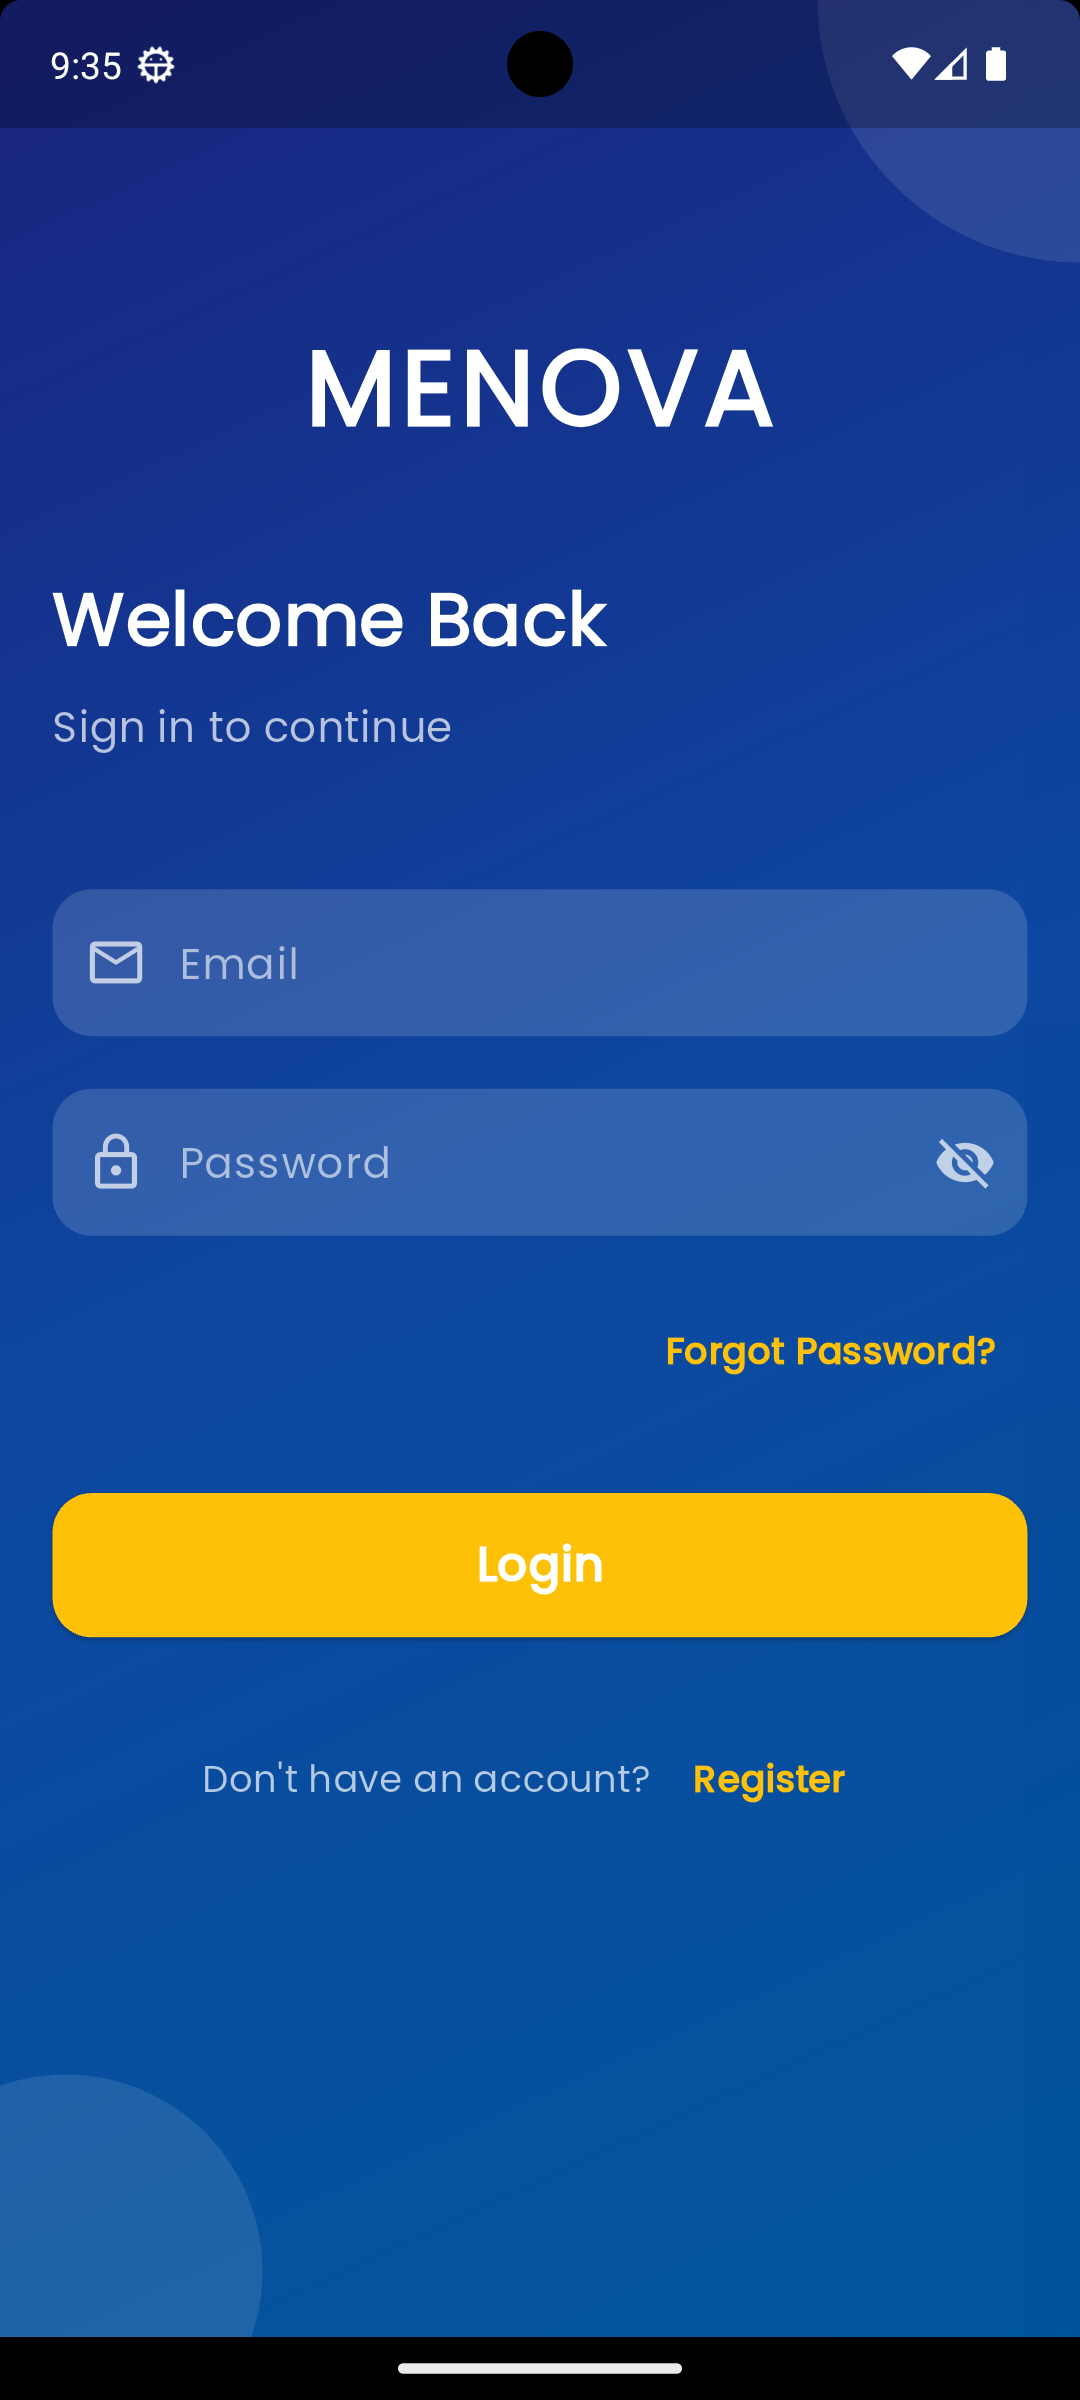
\includegraphics[width=\linewidth, height=0.4\textheight, keepaspectratio]{images/loginMb.png}
        \caption{Interface Mobile – Page de connexion Menova – étape 2}
    \end{minipage}

\end{figure}

\begin{figure}[H]
    \centering

    % Paramètres du cadre
    \setlength{\fboxsep}{2pt}  % espace entre image et cadre
    \setlength{\fboxrule}{0.5pt} % épaisseur du cadre

    % Première rangée : Web + Mobile
    \begin{minipage}[b]{0.6\textwidth}
        \centering
        \fbox{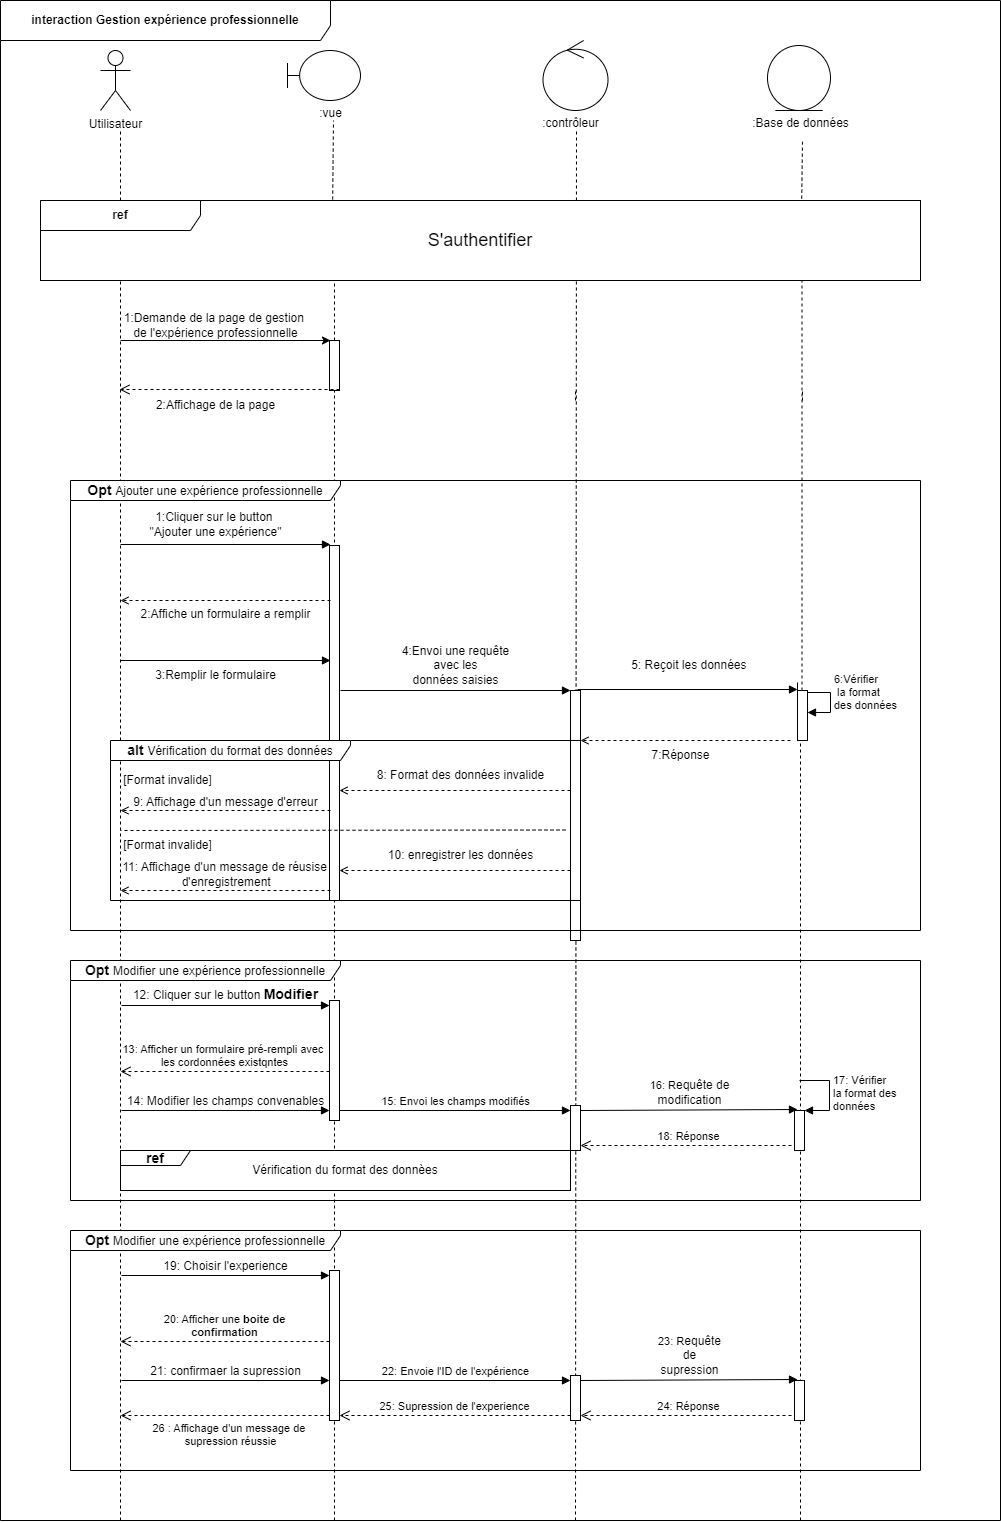
\includegraphics[width=\linewidth, height=0.4\textheight, keepaspectratio]{images/Diagramme gerer profile.png}}
        \caption{Interface Web – Ajouter des expériences ou d’éducations + Modifier Profil – étape 1}
    \end{minipage}
    \hfill
    \begin{minipage}[b]{0.38\textwidth}
        \centering
        \fbox{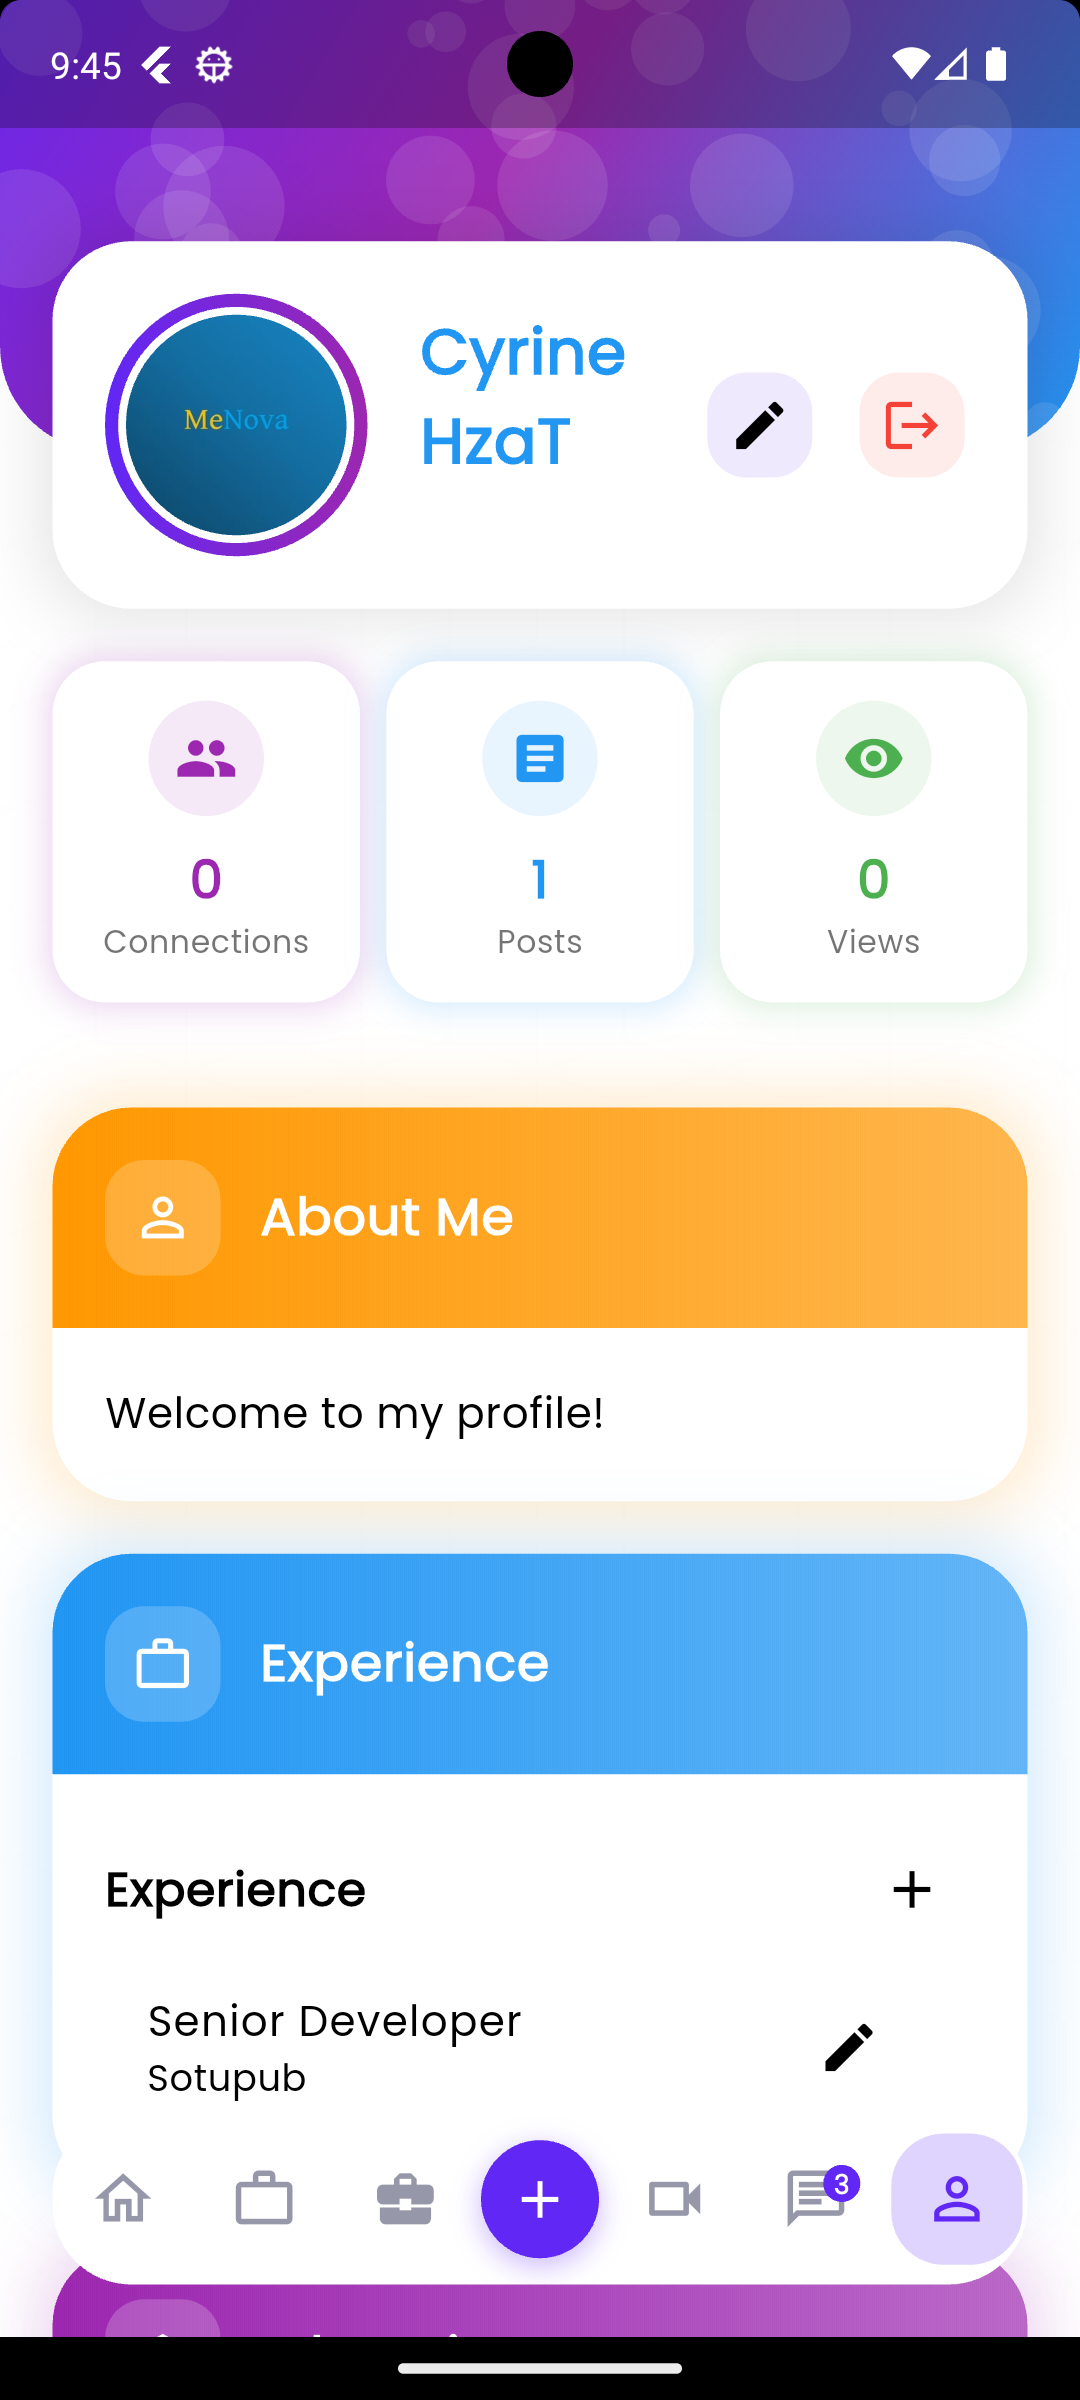
\includegraphics[width=\linewidth, height=0.4\textheight, keepaspectratio]{images/voirProfileMb.png}}
        \caption{Interface Mobile – Voir Profil – étape 2}
    \end{minipage}

    \vspace{1.8em}

    % Deuxième rangée : Web + Mobile
    \begin{minipage}[b]{0.6\textwidth}
        \centering
        \fbox{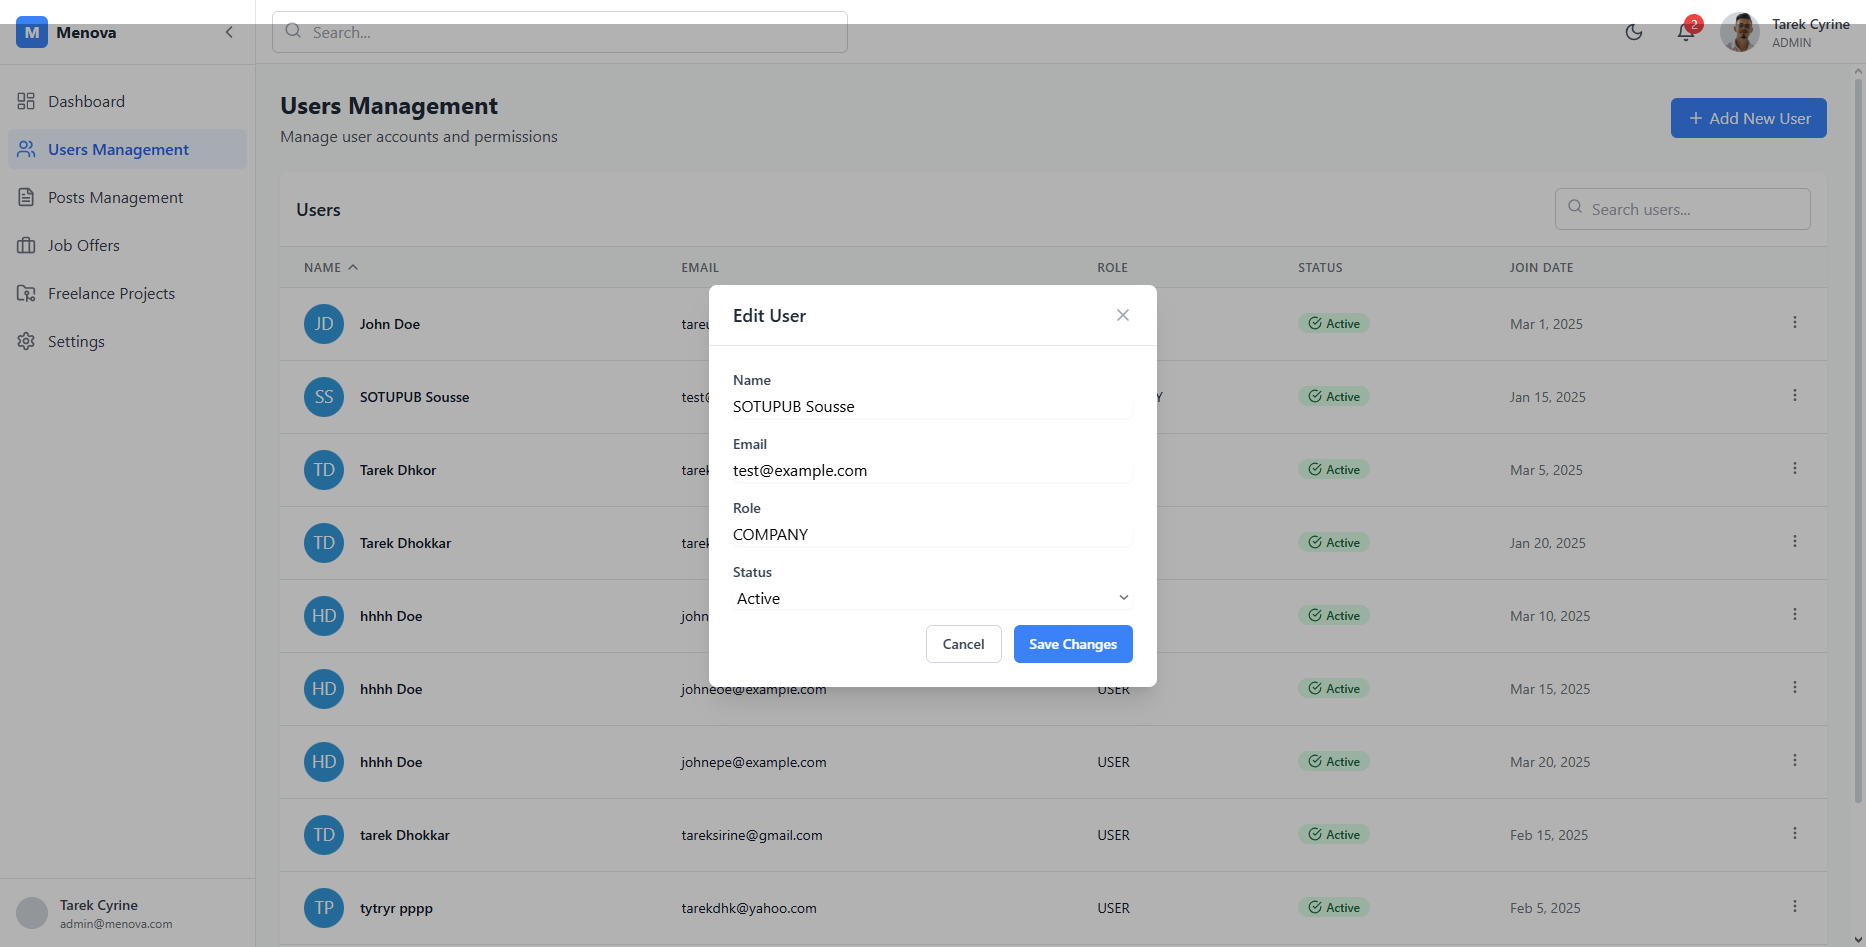
\includegraphics[width=\linewidth, height=0.4\textheight, keepaspectratio]{images/EditUserDashboard.png}}
        \caption{Interface Web – Gérer les utilisateurs – étape 1}
    \end{minipage}
    \hfill
    \begin{minipage}[b]{0.38\textwidth}
        \centering
        \fbox{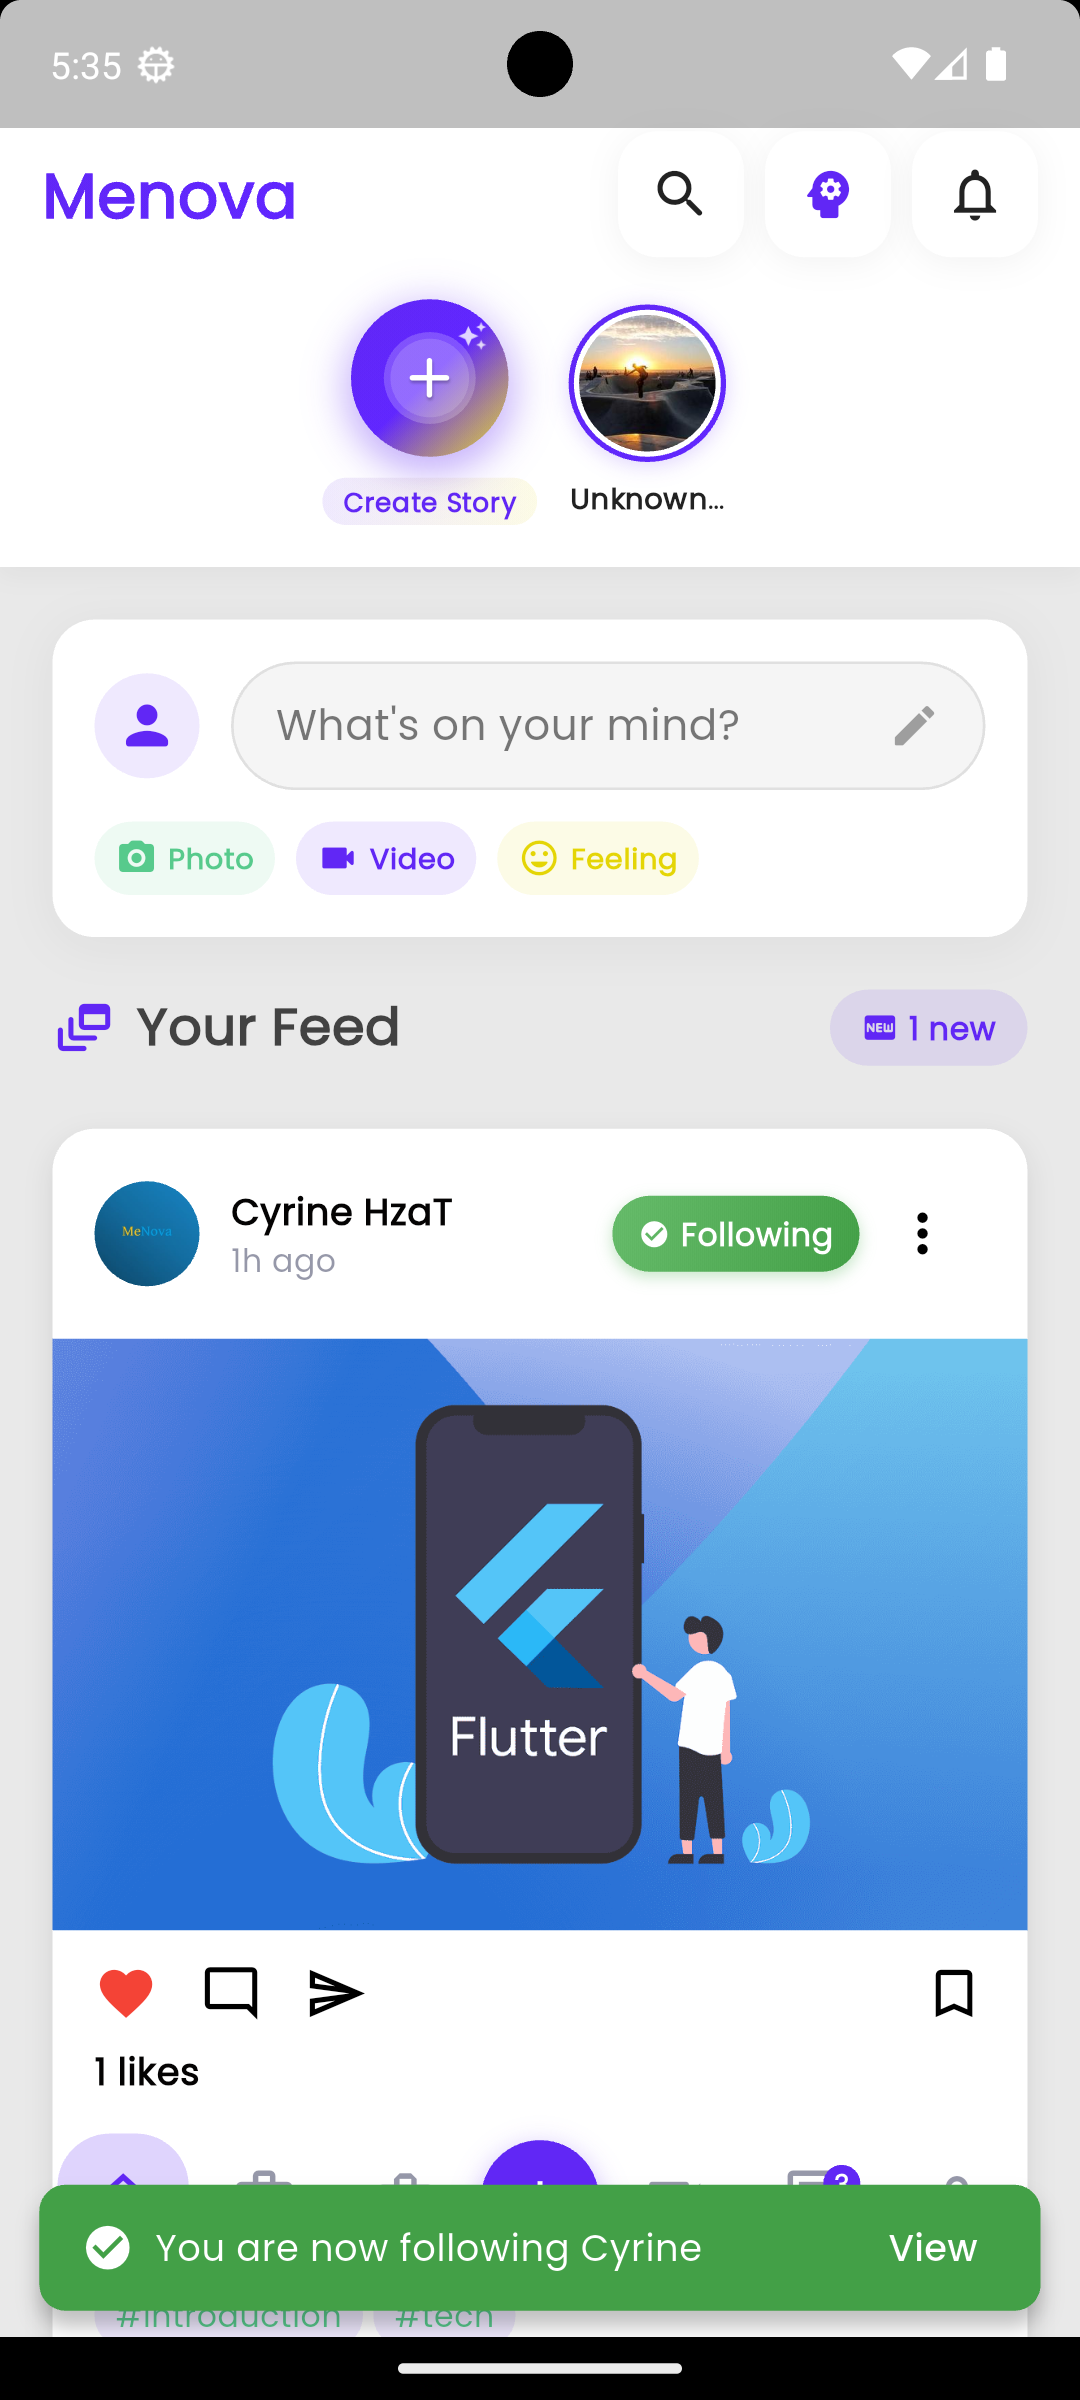
\includegraphics[width=\linewidth, height=0.4\textheight, keepaspectratio]{images/Followetaimerpost.png}}
        \caption{Interface Mobile – Follow un utilisateur – étape 1}
    \end{minipage}

\end{figure}


\newpage
\section*{Conclusion}
\addcontentsline{toc}{section}{Conclusion}
En conclusion, ce chapitre a présenté la mise en place du socle technique de SafeTrack à travers les sprints 1 et 2, notamment l'authentification sécurisée et la gestion des comptes. Ces fondations permettent désormais d'aborder le chapitre suivant, dédié à l'intégration du suivi en temps réel par localisation ainsi qu'au déploiement des systèmes d'alertes et de sécurité SOS .




